\documentclass[crop=false, class=book]{standalone}

\usepackage{lipsum}

\begin{document}
	\chapter{GenomeScope}
	
	Il progetto open source \textit{GenomeScope} cerca sia di stimare le caratteristiche del genoma completo, come la sua lunghezza o il rapporto di eterozigosi, sia di determinare le proprietà delle letture di DNA che prende in input, come la copertura (\textit{read coverage}) o l'error rate~\cite{vurture2017genomescope}. Il programma per determinare tali caratteristiche fa uso del \textit{k-mer profile}, che può essere calcolato tramite programmi specifici, quali \textit{Jellyfish}~\cite{marcais2011fast} o \textit{KMC2}~\cite{deorowicz2015KMC}.
	
	\section{K-mer profile}
	Il k-mer profile, detto anche \textit{k-mer spectrum}, conta la frequenza dei k-mer trovati nelle letture di input, non assemblate o allineate. Esso può rappresentare un indicatore della complessità del genoma preso in esame, come descritto dalla figura~\vref{fig:gnmscp_kmerprofile} tratta da TODO. 
	
	Ipotizzando che le letture siano state fatte senza errori con una certa copertura, se il genoma iniziale è omozigote e senza ripetizioni, il grafico del k-mer profile sarà una distribuzione di Poisson centrata sulla copertura media disponibile; se il genoma è eterozigote invece, il grafico del k-mer profile avrà due picchi in corrispondenza di una certa frequenza e del doppio del suo valore, che rappresentano rispettivamente i k-mer eterozigoti o omozigoti trovati, presenti su uno o su entrambi gli alleli. 
	
	Eventuali ripetizioni aggiungono al grafico ulteriori picchi, mentre errori nelle letture aumentano la varianza e producono distorsioni nel grafico.
	
	\begin{figure}
		\centering
		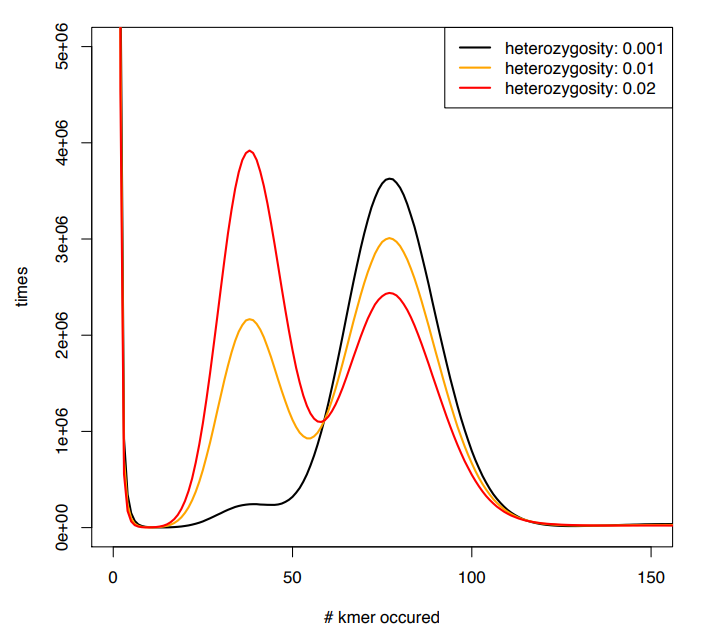
\includegraphics[width=0.6\textwidth]{./resources/images/gnmscp_kmerprofile.png}
		\caption{TODO.}
		\label{fig:gnmscp_kmerprofile}
	\end{figure}

	\section{Algoritmo}
	Il programma effettua una regressione non lineare dei dati del k-mer profile, generando un nuovo profilo che cerca di approssimare il k-mer profile reale. Prendendo in input le letture del genoma che si vuole studiare, esso crea un modello che approssimi il più possibile il k-mer profile. La funzione $f(X)$ scelta per l'interpolazione delle frequenze dei k-mer trovati è la somma di quattro distribuzioni binomiali negative $\mathcal{NB}(X;p,n)$, rispettivamente per rappresentare k-mer eterozigoti trovati nel genoma diploide una volta (unici) o tre volte (duplicati), e k-mer omozigoti di cui si trovano due occorrenze (unici) o trovati quattro volte (duplicati). La funzione $f(X)$ è descritta dall'equazione~\vref{eqn:gnmscp_regression}, in cui $G$ rappresenta un coefficiente di scala legato alla dimensione del genoma, $\lambda$ e $\rho$ sono rispettivamente la media e la varianza della distribuzione. 
	\begin{multline}
		f(X) = G * (\alpha \mathcal{NB}(X;\lambda, \lambda/\rho) + \beta \mathcal{NB}(X;2\lambda, 2\lambda/\rho) + \\
		\gamma \mathcal{NB}(X;3\lambda, 3\lambda/\rho) + \delta \mathcal{NB}(X;4\lambda, 4\lambda/\rho)  )	
		\label{eqn:gnmscp_regression}
	\end{multline}

	I coefficienti $\alpha, \beta, \gamma$ e $\delta$ dipendono dai parametri $r$ e $d$, che rappresentano rispettivamente il rapporto di eterozigosi, cioè la percentuale di basi che sono specifiche a uno o due cromosomi omologhi, e la percentuale del genoma che è presente in due copie.
	
	Lo scopo del programma è quindi determinare i coefficienti $r, d, \lambda$ e $\rho$, oltre alla dimensione totale del genoma $G$. La funzione scelta $f(X)$, tramite cui poi può essere calcolata la dimensione del genoma, è quella che restituisce la minore somma dei quadrati degli errori residui (\textit{Residual Sum of Square Error} - \textit{RSSE}), cioè che minimizzi la somma tra i quadrati degli errori tra i valori osservati e quelli stimati, come descritto dall'equazione~\vref{eqn:gnmscp_RSSE}. Per dedurre i valori dei coefficienti, viene utilizzata la funzione \verb|nls| del linguaggio di programmazione R, che compie la regressione non lineare dei dati alla funzione obiettivo.
	\begin{equation}
		RSSE = \sum_{x=E}^{+\infty} \left(kmer_{obs}[x] - kmer_{pred}[x]\right)^2
	\label{eqn:gnmscp_RSSE}
	\end{equation}
	Al termine, il programma mostra all'utente i dati relativi al genoma trovati, come il rapporto di eterozigosi, la media e la varianza della distribuzione, l'indice RSSE, che rappresenta la percentuale di k-mer non considerati dal modello, e la dimensione stimata del genoma.
	
	Eventuali errori di sequenziamento, ad esempio dovuti a duplicazioni con PCR o a sequenze contaminate, sono determinati solo empiricamente: dopo varie iterazioni del software in cui viene abbassata la soglia di copertura richiesta, i k-mer che non riescono ad essere rappresentati dal modello vengono identificati come errori di sequenziamento. 
	
	\begin{figure}
		\centering
		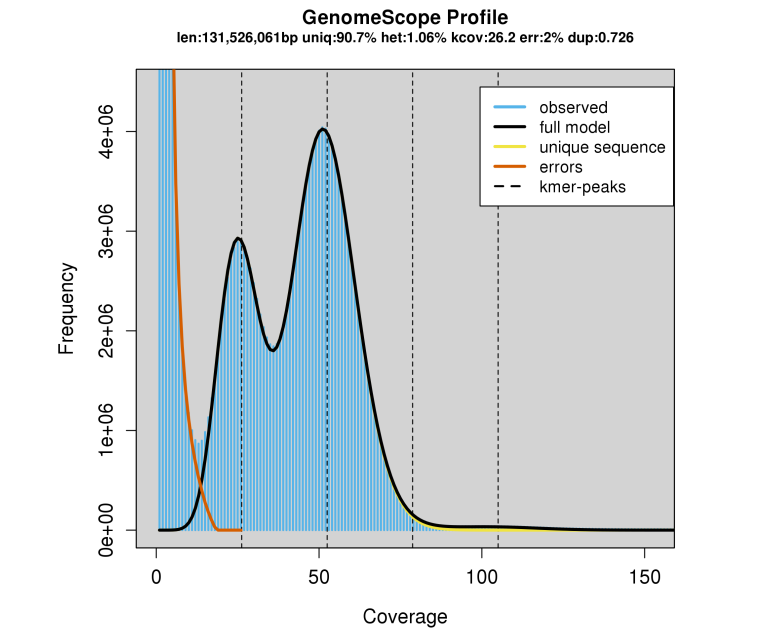
\includegraphics[width=0.6\textwidth]{./resources/images/gnmscp_genomescopeprofile.png}
		\caption{TODO + TODO reference a figura.}
		\label{fig:gnmscp_genomescopeprofile}
	\end{figure}

	%TODO risultati?
	
	%\lipsum[1]
	%\section{Lorem ipsum}
	%\lipsum[2]
	%\subsection{Dolor sit amet} 
	%\lipsum[3]
	%\subsubsection{Lorem ipsum}
	%\lipsum[3]
	
	
	
\end{document}